\documentclass{article}

\usepackage{amsmath}
\usepackage{graphicx}
\graphicspath{ {plots/} }
\title{10-703 Deep Reinforcement Learning and Control \\ Assignment 2 \\}
\date{}

\setlength\parindent{0pt}

\begin{document}

\maketitle

\section*{Problem 1}

Update (1) updates $Q(s,a)$ with $\alpha \Delta Q(s,a)$, where
\begin{align}
  \label{eq:1}
  \Delta Q(s,a) = r + \gamma \max_{a' \in A} Q(s', a') - Q(s,a)
\end{align}

Update (2) updates $w$ with $\alpha \Delta w$, where
\begin{align}
  \label{eq:2}
  \Delta w &= (r + \gamma \max_{a' \in A} Q(s', a') - Q(s,a)) \nabla_{w} Q_{w}(s,a) \\
           &= \Delta Q(s,a) \nabla_{w} Q_{w}(s,a) 
\end{align}

Proving two updates are the same is equivalent to proving
\begin{align}
  \label{eq:3}
  \Delta Q(s,a) = Q_{w+\Delta w}(s,a) - Q_{w}(s,a) 
\end{align}

The RHS is 
\begin{align}
  \label{eq:4}
  Q_{w+\Delta w}(s,a) - Q_{w}(s,a) &= (w + \Delta w)^{T} \phi(s,a) - w^{T} \phi(s,a) \\
                                   &= \Delta w^{T} \phi(s,a) \\
\end{align}

According to \eqref{eq:2},
\begin{align}
  \label{eq:5}
  Q_{w+\Delta w}(s,a) - Q_{w}(s,a) = \Delta Q(s,a) (\nabla_{w} Q_{w}(s,a))^{T} \phi(s,a)\\
\end{align}

While,
\begin{align}
  \label{eq:6}
  \nabla_{w} Q_{w}(s,a) = \nabla_{w} w^{T}\phi(s,a) = \phi(s,a)^{T}
\end{align}

Thus,
\begin{align}
  \label{eq:7}
  Q_{w+\Delta w}(s,a) - Q_{w}(s,a) = \Delta Q(s,a) \phi(s,a)^{T} \phi(s,a)
\end{align}

Given $(s,a)$, $\phi(s,a)$ is an one-hot vector, so $\phi(s,a)^{T} \phi(s,a) = 1$.

Thus, $Q_{w+\Delta w}(s,a) - Q_{w}(s,a) = \Delta Q(s,a)$. 

\section*{Experimental Setup}
We ran all the experiments on SpaceInvaders-v0. The experimental setup is detailed below:

\subsection*{Hyper Parameters}
Discount factor $\gamma$: 0.99\\
Learning rate $\alpha$: 0.0001\\
Epsilon decay policy: start with $\epsilon$=1 and drop it to 0.1 over 1000000 iterations\\
Iterations: 5000000\\
Number of frames to feed: 4\\
Input image size: 84 x 84 x 1\\
Replay buffer size: 1000000\\
Target Q-network reset interval: 10000\\
Batch size: 32\\
Train interval: 4

\subsection*{Configurations}
Optimizer: Adam\\
Loss: Huber loss\\

We used the parameters that were listed in the reference papers for all of our results.

\subsection*{Evaluation Setup}
To evaluate the performance we periodically run the learned policy for 20 episodes every 10000 updates and average the total reward. During evaluation we always choose the best action according to the learned policy.





\section*{Implement a linear Q-network with no experience replay or target fixing}

\section*{Implement a linear Q-network with experience replay and target fixing}

\section*{Implement a linear double Q-network}

\section*{Implement the deep Q-network}
\subsection*{Network model}
The input to the network consists of an 84x84x4 image . The first hidden layer convolves 16 8x8 filters with stride 4 and applies a rectifier nonlinearity. The second layer convolves 32 4x4 filters with stride 2 also followed by rectifier nonlinearity. The final layer is fully connected and consists of 256 rectifier unit. The output layer is a fully connected linear layer with a single output for each action. In case of SpaceInvaders the number of actions is 6.

\begin{figure}[h]
\centering
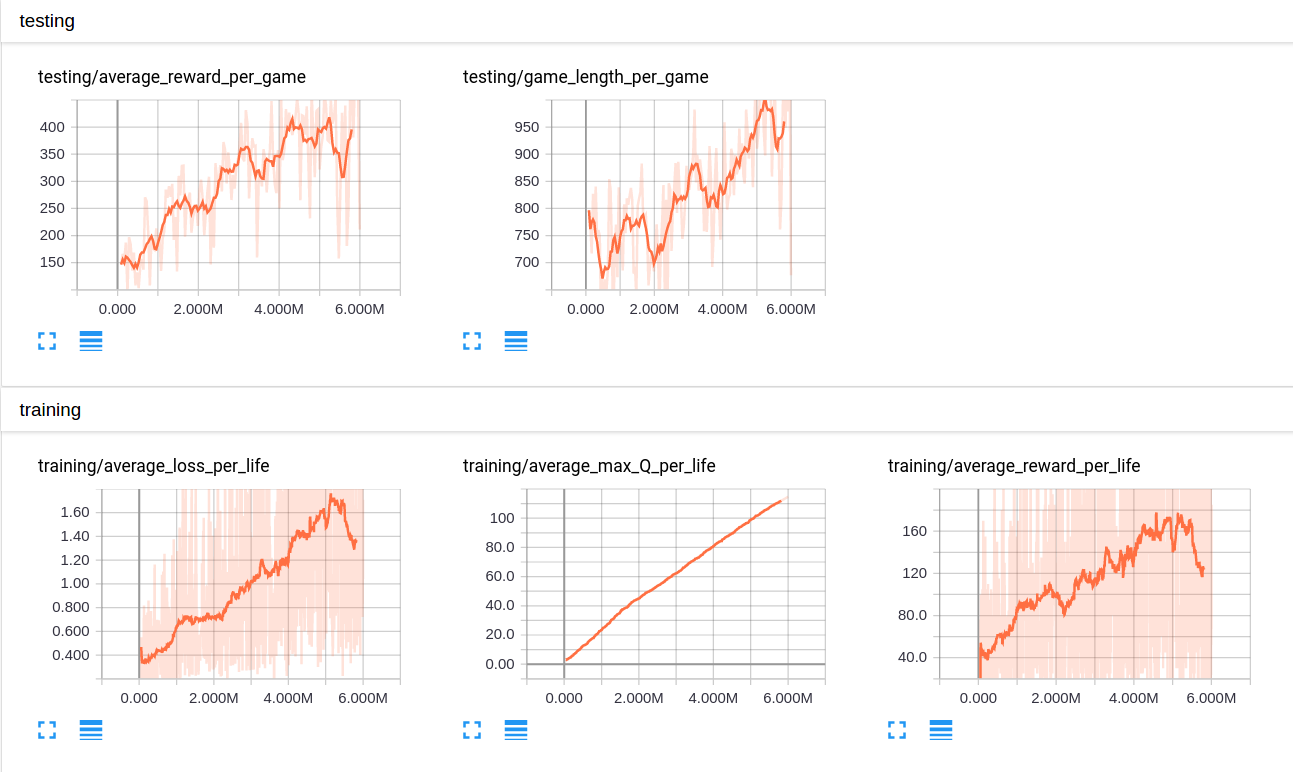
\includegraphics[scale=0.3]{dqn.png}
\end{figure}

\section*{Implement the double deep Q-network}
\subsection*{Network model}
The network architecture we used for double-DQN is the same as we used for DQN. The key algorithmic difference is that it decouples the action selection and evaluation steps to prevent overestimations.

\begin{figure}[h]
\centering
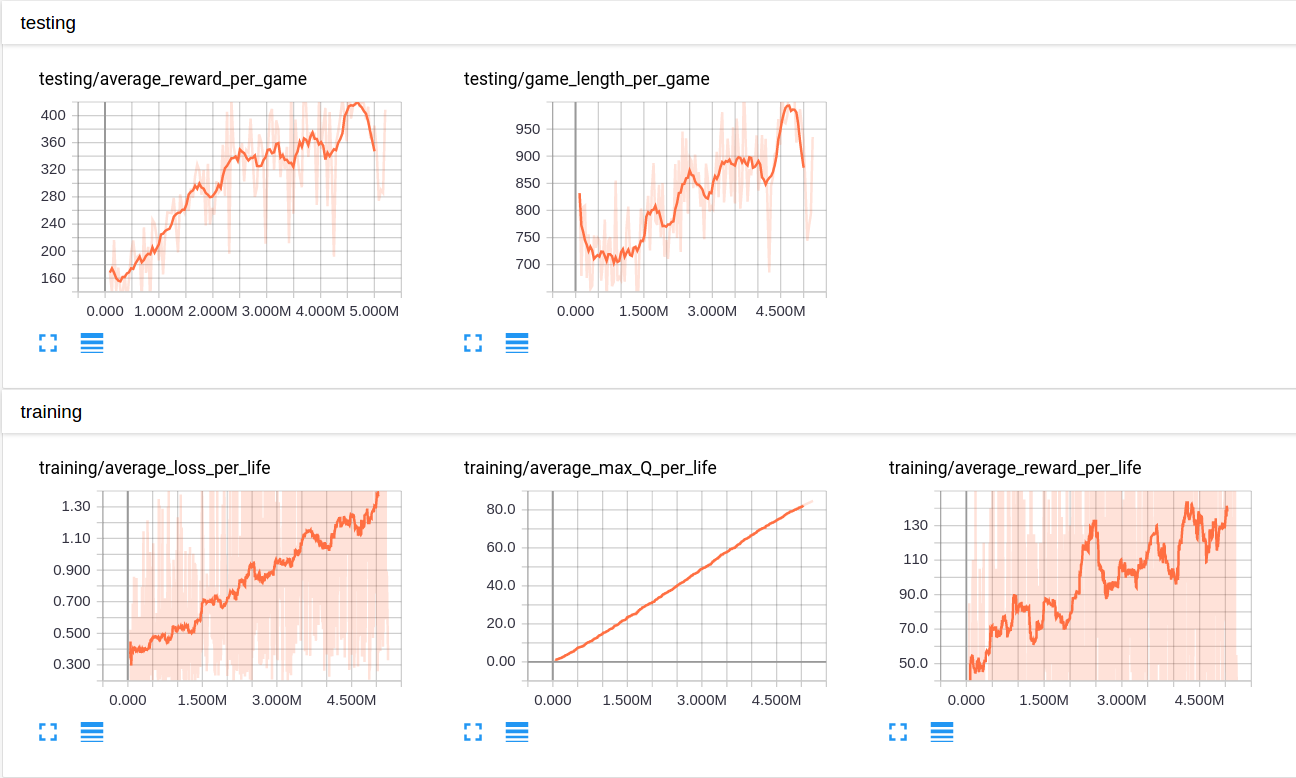
\includegraphics[scale=0.3]{double.png}
\end{figure}

\section*{Implement the dueling deep Q-network}
\subsection*{Network model}
The first three hidden layers for the dueling-DQN are the same as the model we used for DQN. After that the dueling network splits the model into two streams to separately estimate the state-value and the advantages for each action and the two sets of values are finally combined to get the Q-values at the output.

\begin{figure}[h]
\centering
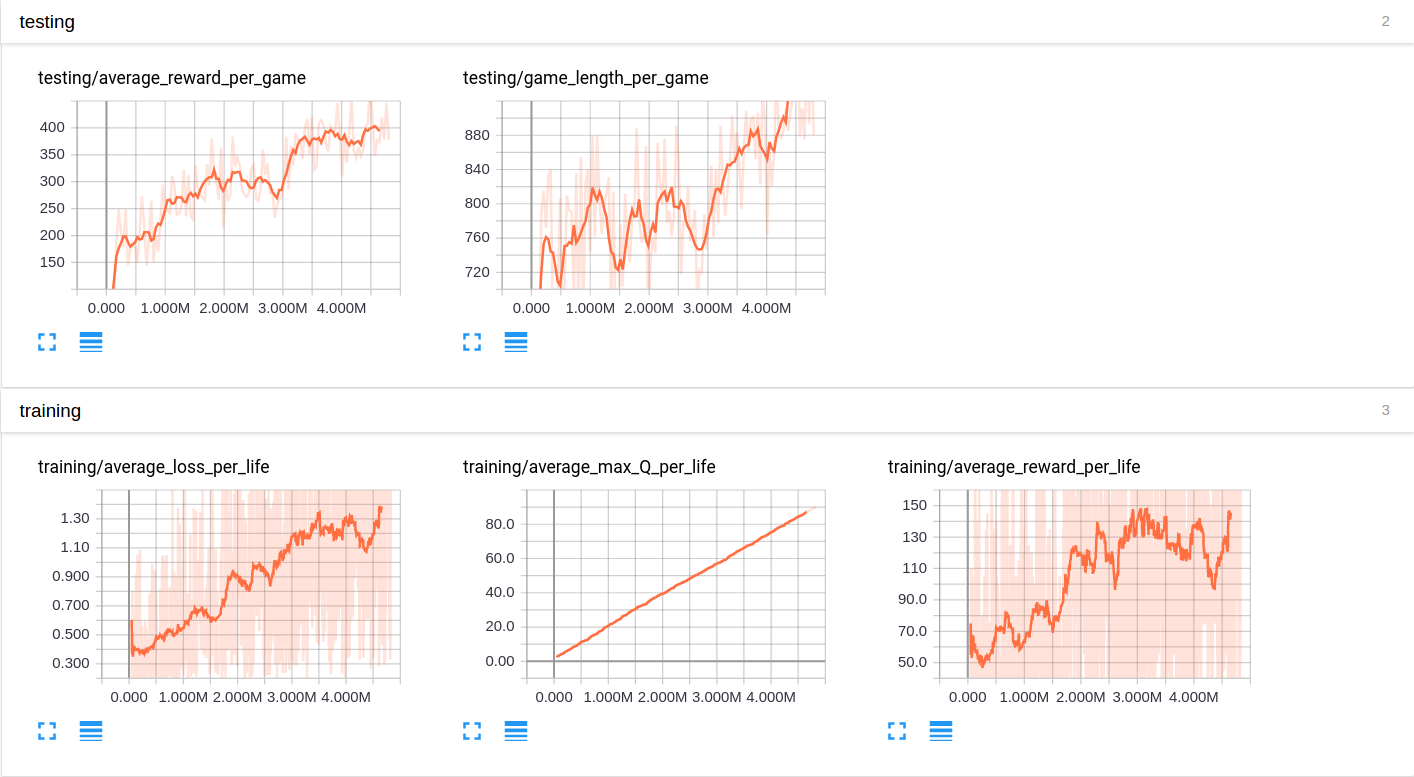
\includegraphics[scale=0.3]{duel.png}
\end{figure}

The table summarizes the average total reward per episode in 100 episodes for the full trained models for all the network models we used for the results.
\begin{center}
 \begin{tabular}{||c | c c||} 
 \hline
 Model & Avg. reward & Mean$\pm$std \\ [0.5ex] 
 \hline\hline
 Linear & 0 & 0 \\ 
 \hline
 Linear* & 0 & 0 \\
 \hline
 double-Linear & 0 & 0 \\
 \hline
 DQN & 0 & 0 \\
 \hline
 double-DQN & 0 & 0 \\  
 \hline
 dueling-DQN & 0 & 0 \\ 
 \hline
\end{tabular}
\end{center}

\end{document}

%%% Local Variables:
%%% mode: latex
%%% TeX-master: t
%%% End:
